\documentclass[border=5mm]{standalone}
\usepackage[utf8]{inputenc}
\usepackage[T1]{fontenc}
\usepackage{tikz}
\usetikzlibrary{shapes.callouts,shadows.blur,decorations.pathmorphing,decorations.pathreplacing,calc,patterns,arrows.meta,positioning}
\usepackage{amsmath,amssymb}
\usepackage{xcolor}

% Color palette
\definecolor{bg}{HTML}{F5F0EB}
\definecolor{panel}{HTML}{FFFFFF}
\definecolor{border}{HTML}{2C3E50}
\definecolor{accent1}{HTML}{E74C3C}  % red
\definecolor{accent2}{HTML}{3498DB}  % blue
\definecolor{accent3}{HTML}{2ECC71}  % green
\definecolor{accent4}{HTML}{F39C12}  % orange
\definecolor{accent5}{HTML}{9B59B6}  % purple
\definecolor{dark}{HTML}{2C3E50}
\definecolor{light}{HTML}{ECF0F1}
\definecolor{ibmblue}{HTML}{0F62FE}
\definecolor{chiralred}{HTML}{C0392B}
\definecolor{chiralorange}{HTML}{E67E22}
\definecolor{boundgold}{HTML}{F1C40F}

\begin{document}
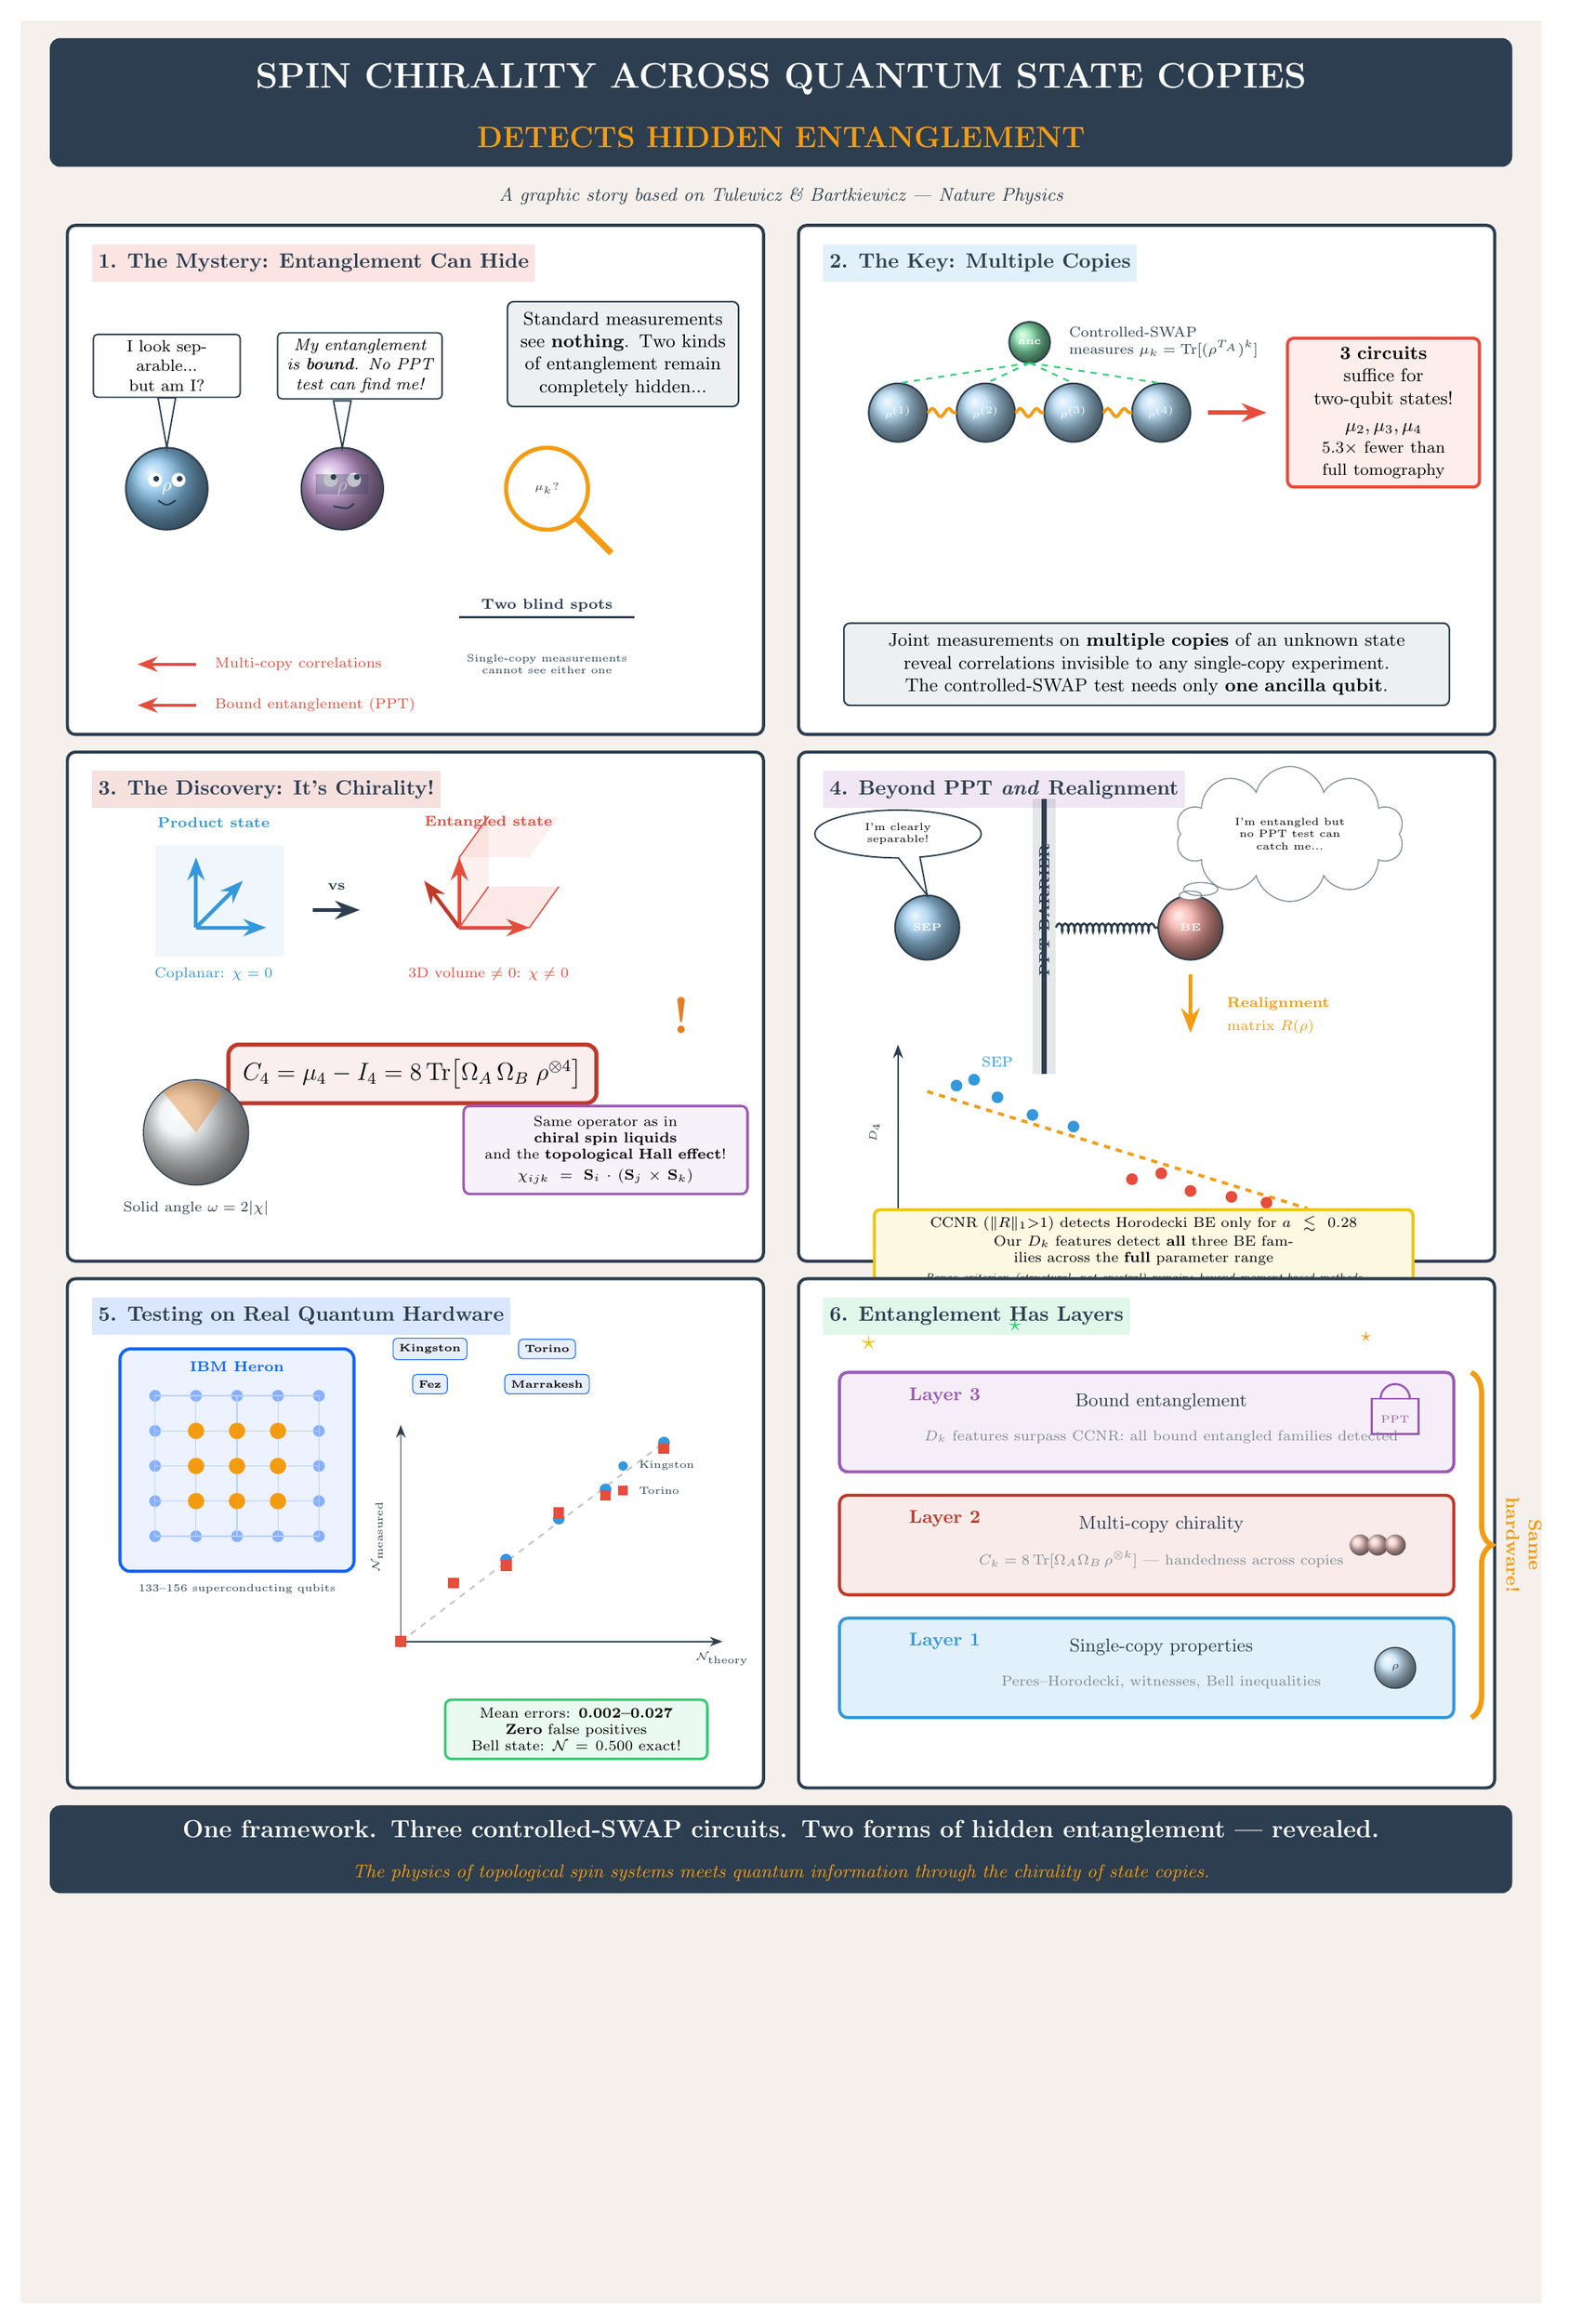
\begin{tikzpicture}[
  panel/.style={draw=border, line width=1.5pt, fill=panel, rounded corners=4pt},
  narrator/.style={fill=light, draw=border, line width=0.8pt, rounded corners=3pt, font=\small, align=center, inner sep=5pt},
  speech/.style={ellipse callout, draw=border, line width=0.7pt, fill=white, font=\footnotesize, callout absolute pointer={#1}, inner sep=3pt, align=center},
  thought/.style={cloud callout, draw=border!60, line width=0.5pt, fill=white, font=\footnotesize\itshape, callout absolute pointer={#1}, inner sep=2pt, align=center, aspect=2.5},
  ptitle/.style={font=\bfseries\normalsize, text=dark},
]

% Background
\fill[bg] (-0.5,-0.5) rectangle (25.5,38.5);

% ============================================================
% TITLE BANNER
% ============================================================
\fill[dark, rounded corners=5pt] (0,36) rectangle (25,38.2);
\node[text=white, font=\bfseries\LARGE] at (12.5,37.5) {SPIN CHIRALITY ACROSS QUANTUM STATE COPIES};
\node[text=accent4, font=\bfseries\Large] at (12.5,36.5) {DETECTS HIDDEN ENTANGLEMENT};

% Author credit
\node[text=dark, font=\itshape\small] at (12.5,35.5) {A graphic story based on Tulewicz \& Bartkiewicz --- Nature Physics};

% ============================================================
% PANEL 1: THE MYSTERY (top-left)
% ============================================================
\draw[panel] (0.3,26.3) rectangle (12.2,35);
\node[ptitle, anchor=north west] at (0.6,34.8) {\colorbox{accent1!15}{\strut 1. The Mystery: Entanglement Can Hide}};

% Two quantum states as cute characters
% State 1 - looking innocent
\shade[ball color=accent2!60] (2,30.5) circle (0.7);
\draw[thick, dark] (2,30.5) circle (0.7);
\node[font=\bfseries\small, text=white] at (2,30.5) {$\rho$};
% Innocent eyes
\fill[white] (1.8,30.65) circle (0.12);
\fill[white] (2.2,30.65) circle (0.12);
\fill[dark] (1.82,30.67) circle (0.05);
\fill[dark] (2.22,30.67) circle (0.05);
% Smile
\draw[dark, thick] (1.85,30.3) .. controls (2,30.2) .. (2.15,30.3);

% State 2 - hiding something (with mask)
\shade[ball color=accent5!60] (5,30.5) circle (0.7);
\draw[thick, dark] (5,30.5) circle (0.7);
\node[font=\bfseries\small, text=white] at (5,30.5) {$\rho$};
% Shifty eyes
\fill[white] (4.8,30.65) circle (0.12);
\fill[white] (5.2,30.65) circle (0.12);
\fill[dark] (4.85,30.7) circle (0.05);
\fill[dark] (5.25,30.7) circle (0.05);
% Mask
\fill[dark, opacity=0.3] (4.55,30.4) -- (5.45,30.4) -- (5.45,30.75) -- (4.55,30.75) -- cycle;
% Smirk
\draw[dark, thick] (4.85,30.2) .. controls (5.1,30.15) .. (5.2,30.25);

% Speech bubble for state 1 (regular rectangle with pointer)
\node[draw=border, line width=0.7pt, fill=white, rounded corners=2pt,
  font=\footnotesize, text width=2.3cm, align=center, inner sep=3pt] (sb1) at (2,32.6) {I look separable...\\but am I?};
\draw[border, line width=0.7pt] (2,31.2) -- (1.85,32.05) -- (2.15,32.05) -- cycle;

% Speech bubble for state 2 (regular rectangle with pointer)
\node[draw=border, line width=0.7pt, fill=white, rounded corners=2pt,
  font=\footnotesize\itshape, text width=2.6cm, align=center, inner sep=3pt] (sb2) at (5.3,32.6) {My entanglement\\is \textbf{bound}. No PPT\\test can find me!};
\draw[border, line width=0.7pt] (5,31.2) -- (4.85,32.0) -- (5.15,32.0) -- cycle;

% Detective magnifying glass
\draw[accent4, line width=2pt] (8.5,30.5) circle (0.7);
\draw[accent4, line width=3pt] (9,30.0) -- (9.6,29.4);
\node[font=\tiny, text=dark] at (8.5,30.5) {$\mu_k$?};

% Narrator box
\node[narrator, text width=3.6cm] at (9.8,32.8) {Standard measurements\\see \textbf{nothing}. Two kinds\\of entanglement remain\\completely hidden...};

% Small icons showing blind spots
\draw[accent1, line width=1.5pt, {Stealth}-] (1.5,27.5) -- (2.5,27.5);
\node[font=\scriptsize, text=accent1, anchor=west] at (2.7,27.5) {Multi-copy correlations};
\draw[accent1, line width=1.5pt, {Stealth}-] (1.5,26.8) -- (2.5,26.8);
\node[font=\scriptsize, text=accent1, anchor=west] at (2.7,26.8) {Bound entanglement (PPT)};

% Barrier icons
\node[font=\scriptsize, text=dark] at (8.5,28.5) {\textbf{Two blind spots}};
\draw[dark, line width=1pt] (7,28.3) -- (10,28.3);
\node[font=\tiny, text=dark, text width=3.5cm, align=center] at (8.5,27.5) {Single-copy measurements\\cannot see either one};

% ============================================================
% PANEL 2: THE KEY IDEA (top-right)
% ============================================================
\draw[panel] (12.8,26.3) rectangle (24.7,35);
\node[ptitle, anchor=north west] at (13.1,34.8) {\colorbox{accent2!15}{\strut 2. The Key: Multiple Copies}};

% Show 4 copies of a state
\foreach \i/\x in {1/14.5, 2/16.0, 3/17.5, 4/19.0} {
  \shade[ball color=accent2!40] (\x,31.8) circle (0.5);
  \draw[thick, dark] (\x,31.8) circle (0.5);
  \node[font=\tiny\bfseries, text=white] at (\x,31.8) {$\rho^{(\i)}$};
}

% SWAP circuit connecting them
\draw[accent4, line width=1.5pt, decorate, decoration={snake, amplitude=2pt, segment length=8pt}]
  (15.0,31.8) -- (15.5,31.8);
\draw[accent4, line width=1.5pt, decorate, decoration={snake, amplitude=2pt, segment length=8pt}]
  (16.5,31.8) -- (17.0,31.8);
\draw[accent4, line width=1.5pt, decorate, decoration={snake, amplitude=2pt, segment length=8pt}]
  (18.0,31.8) -- (18.5,31.8);

% Ancilla qubit
\shade[ball color=accent3!60] (16.75,33.0) circle (0.35);
\draw[thick, dark] (16.75,33.0) circle (0.35);
\node[font=\tiny\bfseries, text=white] at (16.75,33.0) {anc};

% Control lines
\foreach \x in {14.5,16.0,17.5,19.0} {
  \draw[accent3, line width=0.8pt, dashed] (16.75,32.65) -- (\x,32.3);
}

% Label to the right of ancilla
\node[font=\scriptsize, text=dark, text width=3.5cm, align=left, anchor=west] at (17.3,33.0) {Controlled-SWAP\\measures $\mu_k = \mathrm{Tr}[(\rho^{T_A})^k]$};

% Arrow pointing to result
\draw[accent1, line width=2pt, -{Stealth}] (19.8,31.8) -- (20.8,31.8);

% Result box
\node[draw=accent1, line width=1.5pt, fill=accent1!10, rounded corners=3pt,
  font=\small, text width=3cm, align=center, inner sep=4pt] at (22.8,31.8) {
  \textbf{3 circuits}\\suffice for\\two-qubit states!\\[2pt]
  $\mu_2, \mu_3, \mu_4$\\[1pt]
  {\footnotesize $5.3\times$ fewer than\\full tomography}
};

% Narrator
\node[narrator, text width=10cm] at (18.75,27.5) {
  Joint measurements on \textbf{multiple copies} of an unknown state\\
  reveal correlations invisible to any single-copy experiment.\\
  The controlled-SWAP test needs only \textbf{one ancilla qubit}.
};

% ============================================================
% PANEL 3: CHIRALITY (middle-left)
% ============================================================
\draw[panel] (0.3,17.3) rectangle (12.2,26);
\node[ptitle, anchor=north west] at (0.6,25.8) {\colorbox{chiralred!15}{\strut 3. The Discovery: It's Chirality!}};

% Left side: Product state - coplanar spins
\node[font=\scriptsize\bfseries, text=accent2] at (2.8,24.8) {Product state};
% Three coplanar arrows in a flat plane
\draw[-{Stealth}, accent2, line width=1.8pt] (2.5,23) -- (3.7,23);
\draw[-{Stealth}, accent2, line width=1.8pt] (2.5,23) -- (2.5,24.2);
\draw[-{Stealth}, accent2, line width=1.8pt] (2.5,23) -- (3.3,23.8);
% Flat plane shading
\fill[accent2, opacity=0.08] (1.8,22.5) -- (4.0,22.5) -- (4.0,24.4) -- (1.8,24.4) -- cycle;
\node[font=\scriptsize, text=accent2] at (2.8,22.2) {Coplanar: $\chi = 0$};

% Arrow between
\draw[dark, line width=2pt, -{Stealth}] (4.5,23.3) -- (5.3,23.3);
\node[font=\scriptsize\bfseries, text=dark] at (4.9,23.7) {vs};

% Right side: Entangled state - 3D volume
\node[font=\scriptsize\bfseries, text=accent1] at (7.5,24.8) {Entangled state};
% Three non-coplanar arrows
\draw[-{Stealth}, accent1, line width=1.8pt] (7,23) -- (8.2,23);
\draw[-{Stealth}, accent1, line width=1.8pt] (7,23) -- (7,24.2);
\draw[-{Stealth}, chiralred, line width=1.8pt] (7,23) -- (6.4,23.8);
% Parallelepiped faces
\fill[accent1, opacity=0.12] (7,23) -- (8.2,23) -- (8.7,23.7) -- (7.5,23.7) -- cycle;
\fill[accent1, opacity=0.08] (7,23) -- (7,24.2) -- (7.5,24.9) -- (7.5,23.7) -- cycle;
\fill[accent1, opacity=0.08] (7,24.2) -- (8.2,24.2) -- (8.7,24.9) -- (7.5,24.9) -- cycle;
\draw[accent1, line width=0.6pt] (7,23) -- (8.2,23) -- (8.7,23.7);
\draw[accent1, line width=0.6pt] (7,23) -- (7,24.2) -- (7.5,24.9);
\draw[accent1, line width=0.6pt] (7,23) -- (7.5,23.7);
\node[font=\scriptsize, text=accent1] at (7.5,22.2) {3D volume $\neq 0$: $\chi \neq 0$};

% Central equation with prominent box
\node[draw=chiralred, line width=2pt, fill=chiralred!8, rounded corners=5pt,
  inner sep=7pt, font=\large] at (6.2,20.5) {
  $C_4 = \mu_4 - I_4 = 8\,\mathrm{Tr}\bigl[\Omega_A\,\Omega_B\;\rho^{\otimes 4}\bigr]$
};

% Exclamation
\node[font=\Huge, text=chiralorange] at (10.8,21.5) {\textbf{!}};

% Connection to condensed matter
\node[draw=accent5, line width=1.2pt, fill=accent5!8, rounded corners=3pt,
  font=\scriptsize, text width=4.5cm, align=center, inner sep=5pt] at (9.5,19.2) {
  Same operator as in\\
  \textbf{chiral spin liquids}\\
  and the \textbf{topological Hall effect}!\\[2pt]
  $\chi_{ijk} = \mathbf{S}_i \cdot (\mathbf{S}_j \times \mathbf{S}_k)$
};

% Mini Bloch sphere
\shade[ball color=light] (2.5,19.5) circle (0.9);
\draw[dark, line width=0.5pt] (2.5,19.5) circle (0.9);
% Solid angle wedge
\fill[chiralorange, opacity=0.4] (2.5,19.5) -- (2.95,20.15) arc (45:130:0.75) -- cycle;
\node[font=\scriptsize, text=dark] at (2.5,18.2) {Solid angle $\omega = 2|\chi|$};

% ============================================================
% PANEL 4: BOUND ENTANGLEMENT (middle-right)
% ============================================================
\draw[panel] (12.8,17.3) rectangle (24.7,26);
\node[ptitle, anchor=north west] at (13.1,25.8) {\colorbox{accent5!15}{\strut 4. Beyond PPT \emph{and} Realignment}};

% PPT Barrier wall
\fill[dark, opacity=0.12] (16.8,20.5) rectangle (17.2,25.2);
\draw[dark, line width=2.5pt] (17,20.5) -- (17,25.2);
\node[font=\scriptsize\bfseries, text=dark, rotate=90] at (17,23.3) {PPT BARRIER};

% Separable state (left of barrier)
\shade[ball color=accent2!50] (15,23) circle (0.55);
\draw[thick, dark] (15,23) circle (0.55);
\node[font=\tiny\bfseries, text=white] at (15,23) {SEP};
\node[speech={(15,23.55)}, text width=1.8cm, font=\tiny] at (14.5,24.6) {I'm clearly\\separable!};

% Bound entangled state (right of barrier, trapped)
\shade[ball color=accent1!50] (19.5,23) circle (0.55);
\draw[thick, dark] (19.5,23) circle (0.55);
\node[font=\tiny\bfseries, text=white] at (19.5,23) {BE};
% Chain
\draw[dark, line width=1pt, decorate, decoration={coil, aspect=0.4, segment length=3pt, amplitude=2pt}]
  (17.2,23) -- (18.95,23);
\node[thought={(19.5,23.55)}, text width=2.5cm, font=\tiny] at (21.2,24.6) {I'm entangled but\\no PPT test can\\catch me...};

% The solution arrow
\draw[accent4, line width=2pt, -{Stealth}] (19.5,22.2) -- (19.5,21.2);
\node[font=\scriptsize\bfseries, text=accent4, anchor=west] at (20,21.7) {Realignment};
\node[font=\scriptsize, text=accent4, anchor=west] at (20,21.3) {matrix $R(\rho)$};

% Feature space scatter plot
\draw[dark, line width=0.8pt, -{Stealth}] (14.5,18) -- (21.8,18);
\draw[dark, line width=0.8pt, -{Stealth}] (14.5,18) -- (14.5,21);
\node[font=\tiny, text=dark] at (22,17.7) {$\Sigma_2^2/\Sigma_4$};
\node[font=\tiny, text=dark, rotate=90] at (14.1,19.5) {$D_4$};

% Decision boundary
\draw[accent4, line width=1.5pt, dashed] (15,20.2) -- (21.5,18.2);

% Separable points (above line)
\foreach \x/\y in {15.5/20.3, 16.2/20.1, 16.8/19.8, 15.8/20.4, 17.5/19.6} {
  \fill[accent2] (\x,\y) circle (0.1);
}
% BE points (below line)
\foreach \x/\y in {18.5/18.7, 19.5/18.5, 20.2/18.4, 19/18.8, 20.8/18.3} {
  \fill[accent1] (\x,\y) circle (0.1);
}

% Labels in plot
\node[font=\scriptsize, text=accent2] at (16.2,20.7) {SEP};
\node[font=\scriptsize, text=accent1] at (20,18.1) {BE};

% Key insight box
\node[draw=boundgold, line width=1.5pt, fill=boundgold!12, rounded corners=3pt,
  font=\scriptsize, text width=9cm, align=center, inner sep=3pt] at (18.7,17.5) {
  CCNR ($\|R\|_1 {>} 1$) detects Horodecki BE only for $a \lesssim 0.28$\\[1pt]
  Our $D_k$ features detect \textbf{all} three BE families across the \textbf{full} parameter range\\[1pt]
  {\tiny\itshape Range criterion (structural, not spectral) remains beyond moment-based methods}
};

% ============================================================
% PANEL 5: THE EXPERIMENT (bottom-left)
% ============================================================
\draw[panel] (0.3,8.3) rectangle (12.2,17);
\node[ptitle, anchor=north west] at (0.6,16.8) {\colorbox{ibmblue!15}{\strut 5. Testing on Real Quantum Hardware}};

% IBM chip illustration
\fill[ibmblue!8, rounded corners=5pt] (1.2,12) rectangle (5.2,15.8);
\draw[ibmblue, line width=1.5pt, rounded corners=5pt] (1.2,12) rectangle (5.2,15.8);

% Grid of qubits
\foreach \x in {1.8, 2.5, 3.2, 3.9, 4.6} {
  \foreach \y in {12.6, 13.2, 13.8, 14.4, 15.0} {
    \fill[ibmblue!50] (\x,\y) circle (0.1);
  }
}
% Horizontal connections
\foreach \x in {1.8, 2.5, 3.2, 3.9} {
  \foreach \y in {12.6, 13.2, 13.8, 14.4, 15.0} {
    \draw[ibmblue!30, line width=0.4pt] (\x,\y) -- (\x+0.7,\y);
  }
}
% Vertical connections
\foreach \x in {1.8, 2.5, 3.2, 3.9, 4.6} {
  \foreach \y in {12.6, 13.2, 13.8, 14.4} {
    \draw[ibmblue!30, line width=0.4pt] (\x,\y) -- (\x,\y+0.6);
  }
}

% Highlight active qubits (9 = 4-copy 2-qubit + ancilla)
\foreach \x/\y in {2.5/14.4, 3.2/14.4, 3.9/14.4, 2.5/13.8, 3.2/13.8, 3.9/13.8, 2.5/13.2, 3.2/13.2, 3.9/13.2} {
  \fill[accent4] (\x,\y) circle (0.14);
}

\node[font=\scriptsize\bfseries, text=ibmblue] at (3.2,15.5) {IBM Heron};
\node[font=\tiny, text=dark] at (3.2,11.7) {133--156 superconducting qubits};

% Four processor name badges
\node[draw=ibmblue, fill=ibmblue!10, rounded corners=2pt, font=\tiny\bfseries, inner sep=3pt] at (6.5,15.8) {Kingston};
\node[draw=ibmblue, fill=ibmblue!10, rounded corners=2pt, font=\tiny\bfseries, inner sep=3pt] at (8.5,15.8) {Torino};
\node[draw=ibmblue, fill=ibmblue!10, rounded corners=2pt, font=\tiny\bfseries, inner sep=3pt] at (6.5,15.2) {Fez};
\node[draw=ibmblue, fill=ibmblue!10, rounded corners=2pt, font=\tiny\bfseries, inner sep=3pt] at (8.5,15.2) {Marrakesh};

% Results mini-plot (negativity)
\draw[dark, line width=0.7pt, -{Stealth}] (6,10.8) -- (11.5,10.8);
\draw[dark, line width=0.7pt, -{Stealth}] (6,10.8) -- (6,14.5);
\node[font=\tiny, text=dark] at (11.5,10.5) {$\mathcal{N}_{\mathrm{theory}}$};
\node[font=\tiny, text=dark, rotate=90] at (5.6,12.6) {$\mathcal{N}_{\mathrm{measured}}$};

% Perfect agreement line
\draw[dark!30, line width=0.8pt, dashed] (6,10.8) -- (10.5,14.2);

% Data points Kingston (blue circles)
\foreach \x/\y in {6/10.8, 7.8/12.2, 8.7/12.9, 9.5/13.4, 10.5/14.2} {
  \fill[accent2] (\x,\y) circle (0.1);
}
% Data points Torino (red squares)
\foreach \x/\y in {6/10.8, 6.9/11.8, 7.8/12.1, 8.7/13, 9.5/13.3, 10.5/14.1} {
  \draw[accent1, line width=0.8pt] (\x-0.08,\y-0.08) rectangle (\x+0.08,\y+0.08);
  \fill[accent1] (\x-0.08,\y-0.08) rectangle (\x+0.08,\y+0.08);
}

% Legend
\fill[accent2] (9.8,13.8) circle (0.08);
\node[font=\tiny, text=dark, anchor=west] at (9.95,13.8) {Kingston};
\fill[accent1] (9.72,13.3) rectangle (9.88,13.46);
\node[font=\tiny, text=dark, anchor=west] at (9.95,13.38) {Torino};

% Results highlight box
\node[draw=accent3, line width=1.2pt, fill=accent3!10, rounded corners=3pt,
  font=\scriptsize, text width=4.2cm, align=center, inner sep=4pt] at (9,9.3) {
  Mean errors: \textbf{0.002--0.027}\\
  \textbf{Zero} false positives\\
  Bell state: $\mathcal{N} = 0.500$ exact!
};

% ============================================================
% PANEL 6: THE PUNCHLINE (bottom-right)
% ============================================================
\draw[panel] (12.8,8.3) rectangle (24.7,17);
\node[ptitle, anchor=north west] at (13.1,16.8) {\colorbox{accent3!15}{\strut 6. Entanglement Has Layers}};

% Three layers as stacked platforms
% Layer 1 - Single copy (bottom)
\fill[accent2!15, rounded corners=4pt] (13.5,9.5) rectangle (24,11.2);
\draw[accent2, line width=1.5pt, rounded corners=4pt] (13.5,9.5) rectangle (24,11.2);
\node[font=\small\bfseries, text=accent2] at (15.3,10.8) {Layer 1};
\node[font=\small, text=dark] at (19,10.7) {Single-copy properties};
\node[font=\scriptsize, text=dark!60] at (19,10.1) {Peres--Horodecki, witnesses, Bell inequalities};
% icon
\shade[ball color=accent2!30] (23,10.35) circle (0.35);
\draw[dark, line width=0.5pt] (23,10.35) circle (0.35);
\node[font=\tiny, text=dark] at (23,10.35) {$\rho$};

% Layer 2 - Chirality (middle)
\fill[chiralred!10, rounded corners=4pt] (13.5,11.6) rectangle (24,13.3);
\draw[chiralred, line width=1.5pt, rounded corners=4pt] (13.5,11.6) rectangle (24,13.3);
\node[font=\small\bfseries, text=chiralred] at (15.3,12.9) {Layer 2};
\node[font=\small, text=dark] at (19,12.8) {Multi-copy chirality};
\node[font=\scriptsize, text=dark!60] at (19,12.2) {$C_k = 8\,\mathrm{Tr}[\Omega_A\Omega_B\,\rho^{\otimes k}]$ --- handedness across copies};
% icon: 3 connected copies
\foreach \dx in {-0.3,0,0.3} {
  \shade[ball color=chiralred!30] (22.7+\dx,12.45) circle (0.18);
}

% Layer 3 - Bound entanglement (top)
\fill[accent5!10, rounded corners=4pt] (13.5,13.7) rectangle (24,15.4);
\draw[accent5, line width=1.5pt, rounded corners=4pt] (13.5,13.7) rectangle (24,15.4);
\node[font=\small\bfseries, text=accent5] at (15.3,15) {Layer 3};
\node[font=\small, text=dark] at (19,14.9) {Bound entanglement};
\node[font=\scriptsize, text=dark!60] at (19,14.3) {$D_k$ features surpass CCNR: all bound entangled families detected};
% icon: lock
\draw[accent5, line width=1pt] (22.6,14.35) rectangle (23.4,14.95);
\draw[accent5, line width=1pt] (22.75,14.95) arc (180:0:0.25) -- (23.25,14.95);
\node[font=\tiny, text=accent5] at (23,14.6) {PPT};

% Connecting bracket
\draw[accent4, line width=2.5pt, decorate, decoration={brace, amplitude=10pt, mirror}]
  (24.3,9.5) -- (24.3,15.4);
\node[font=\small\bfseries, text=accent4, rotate=-90, text width=3cm, align=center] at (25.2,12.45) {Same\\hardware!};

% Decorative stars
\node[font=\Large, text=boundgold] at (14,15.9) {$\star$};
\node[font=\normalsize, text=accent4] at (22.5,16) {$\star$};
\node[font=\large, text=accent3] at (16.5,16.2) {$\star$};

% ============================================================
% BOTTOM BANNER
% ============================================================
\fill[dark, rounded corners=5pt] (0,6.5) rectangle (25,8);
\node[text=white, font=\bfseries\large, text width=24cm, align=center] at (12.5,7.55) {
  One framework. Three controlled-SWAP circuits. Two forms of hidden entanglement --- revealed.
};
\node[text=accent4, font=\small\itshape, text width=24cm, align=center] at (12.5,6.85) {
  The physics of topological spin systems meets quantum information through the chirality of state copies.
};

\end{tikzpicture}
\end{document}
